% !TEX TS-program = pdflatex
% !TEX encoding = UTF-8 Unicode

% This is a simple template for a LaTeX document using the "article" class.
% See "book", "report", "letter" for other types of document.

\documentclass[12pt]{article} % use larger type; default would be 10pt

\usepackage[utf8]{inputenc} % set input encoding (not needed with XeLaTeX)

%%% Examples of Article customizations
% These packages are optional, depending whether you want the features they provide.
% See the LaTeX Companion or other references for full information.

%%% PAGE DIMENSIONS
\usepackage{geometry} % to change the page dimensions
\geometry{a4paper} % or letterpaper (US) or a5paper or....
% \geometry{margin=2in} % for example, change the margins to 2 inches all round
% \geometry{landscape} % set up the page for landscape
%   read geometry.pdf for detailed page layout information

\usepackage{graphicx} % support the \includegraphics command and options

%%% PACKAGES
\usepackage{booktabs} % for much better looking tables
\usepackage{array} % for better arrays (eg matrices) in maths
\usepackage{paralist} % very flexible & customisable lists (eg. enumerate/itemize, etc.)
\usepackage{verbatim} % adds environment for commenting out blocks of text & for better verbatim
\usepackage{subfig} % make it possible to include more than one captioned figure/table in a single float
\usepackage{pdfpages}
\usepackage{amsmath,mathtools,amsfonts}
\usepackage{bm}
\usepackage{blindtext}
\usepackage{fancyhdr}
\usepackage{float}
\usepackage{gensymb}
\usepackage{svg}

\graphicspath{ {./images/} }

%%% HEADERS & FOOTERS
\pagestyle{fancy}
\renewcommand{\headrulewidth}{1pt} % customise the layout...
\renewcommand{\footrulewidth}{1pt} % customise the layout...
\renewcommand{\sectionmark}[1]{\markright{#1}}
\fancyhf{}

% HEADER
\fancyhead[L]{ENEL321 Lab Report}
\fancyhead[C]{Jesse Sheehan}
\fancyhead[R]{\nouppercase{\rightmark}}

% FOOTER
\fancyfoot[L]{\reflectbox{\includesvg[width=12pt]{rocket}}}
\fancyfoot[C]{\thepage}
\fancyfoot[R]{\includesvg[width=12pt]{rocket}}

%% TITLE
\title{\uppercase{
	Design, Implementation and Analysis of a Control System
}}
\date{\today}
\author{
	Jesse Patrick Sheehan\\
	\\
	{\small{ID: 53366509}}\\
	{\small{jps111@uclive.ac.nz}}\\
}

%\renewcommand{\sectionmark}[1]{\markright{\thesection\ #1}}

\begin{document}

\maketitle

\vfill

\renewcommand{\abstractname}{Executive Summary}

\begin{abstract}

% Motivation, what was done, summary of results (very brief)

\blindtext

\end{abstract}

\newpage

\section{Methodology}

% Briefly introduce the problem, and experiment but don't derive the model.
A test rig (see figure \ref{fig:test-rig}) controlled by two brushless DC motors is subjected to a 20\degree\ step input.

\begin{figure}[H]
	\centering
	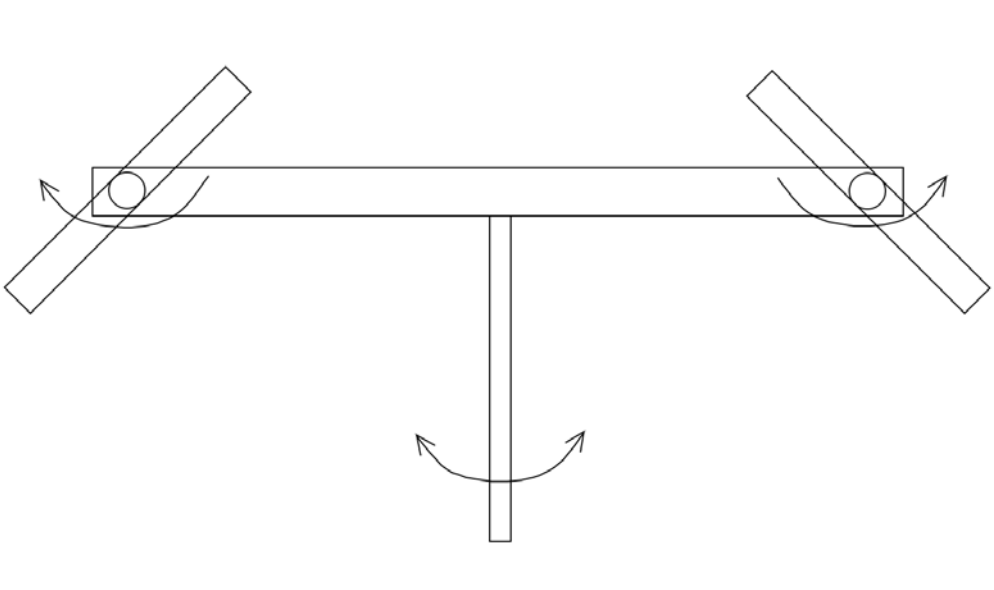
\includegraphics[scale=0.8]{test-rig}
	\caption{A front view of the test rig system (Hann, 2019).}
	\label{fig:test-rig}
\end{figure}

\noindent A feedback control system was designed and implemented to meet the following design specifications:
\begin{align*}
\xi &> 0.1 & M_p\% &< 15\%  \\[1em]
e_{ss} &< 1.5\degree & t_r &< 0.8 \textrm{s} \\[1em]
1 \leq K_p &\leq 2.5 & \frac{K_d}{K_p} &< 0.7
\end{align*}

% Explain how you designed your gains, and what values you used and why.
\noindent The predetermined gain values were found using an iterative approach. The transfer function (see equation\ \ref{eq:transfer-function}), with the suggested parameters $\alpha = 1.6$, $\beta = 2.9$, $\gamma = 1.3$ and $\tau = 0.34$, was used with MATLAB to predict how output would be affected by the gains and the step input.
\\ 

\begin{equation}
\label{eq:transfer-function}
\frac{X}{R} = \frac{\beta K_p s + \beta K_i}{s^3 + s^2 (\alpha + \beta K_d - \beta K_p \tau) + s(\gamma + \beta K_p - \beta K_i \tau) + \beta K_i}
\end{equation}
\\ 

\noindent Three sets of predetermined gain values were ultimately decided on:
\begin{align*}
\textrm{P Controller} &: & K_p &= 1.20 & & & \\[1em]
\textrm{PD Controller} &: & K_p &= 1.20 & K_d &= 1.20 & & \\[1em]
\textrm{PID Controller} &: & K_p &= 1.20 & K_d &= 0.72 & K_i &= 0.84
\end{align*}

% Explain the different controllers used.
\noindent By using three different controllers, we were able to analyse the differences between them and to better understand the relationship between the step input, the gains, and the output.
\\ 

\noindent The P Controller would be expected to overshoot the target angle and then overshoot in the other direction, oscillating until it comes to a rest near the target angle. This would be an example of an underdamped system.
The PD Controller would be expected to slowly converge upon the target angle with little or no overshoot (depending on the damping coefficient). A relatively large steady-state error ($e_{ss}$) would be expected. This would be an example of an overdamped system.
The PID Controller is expected to overshoot but then quickly converge towards the target angle. This would be an example of a critically damped system.

\section{Results}

% Present experimental results.



\newpage

\section{Discussion}

% Compare results with model, explain differences.
% Focus on the why rather than the what.

\blindtext

\blindtext

\blindtext

\newpage

\section{Conclusion}

% Summarize what worked and what didn't, what could be improved as well as any limitations in the methods observed.

\blindtext

\blindtext

\blindtext

\end{document}
